\chapter{ПРОВЕРКА ВЫЧИСЛИТЕЛЬНОЙ ПРОГРАММЫ} \label{ch4}

\section{Инициализация плазмы}

\subsection{Задание начальных положений}
\label{sec:MT19937}

Для того чтобы правильно инициализировать систему необходимо выработать алгоритм случайного задания \textit{положений} и \textit{скоростей}. 

Задача задания случайного положения решается путём выбора наиболее хорошего генератора псевдослучайных чисел. Был выбран генератор вихрь Мерсенна с его алгоритмической реализацией MT19937. Причины выбора следующие: данный алгоритм обеспечивает быструю и очень качественную реализацию генерации псевдослучайных чисел. Его период составляет $2^{19937}-1$, а также алгоритм показывает высокие результаты в тесте DIEHARD \cite{matsumoto1998mersenne,sriram2006area}.

Стоить заметить, что использование стандартной функции \texttt{RAND()} в \texttt{c++} неприменимо, т.~к. тогда наблюдаются определенные неслучайные пространственные структуры, что недопустимо \cite{habr_rand}.

\subsection{Задание начальных скоростей согласно распределению Максвелла}
\label{sec:HowToMaxwell}

Для частиц в плазме справедливо распределение Максвелла (за некоторыми частными исключениями). Встаёт задача о задании процедуры случайного задания скорости по заданной функции плотности распределения:
\begin{equation}
f(v) = 4 \pi v^2 \left( \frac{m}{2 \pi T} \right)^{3/2} \exp \left[ - \frac{m v^2/2}{T} \right].
\label{eq:maxwell_dist}
\end{equation}

Алгоритм решения поставленной задачи следующий:
\begin{enumerate}
\item Зная конкретный вид $f(v)$, численно табулируется функция распределения
\begin{equation}
F_i (v_i) = \int\limits_{- \infty}^{v_i} f(v') dv'.
\end{equation}
\item По данным таблицы значений $\left\{ F_i ; v_i  \right\}$, интерполируется функция  $F^{-1}(v) = v(F)$.
\item В силу свойств функции распределения $F \in \left[0,1\right]$. Тогда, очевидно, необходимо задать случайную величину в диапазоне от 0 до 1, подставить в полученную функцию и получить желаемый результат (рисунок \ref{fig:He(T=273)}).
\end{enumerate}

\begin{figure}[h!]
\centering
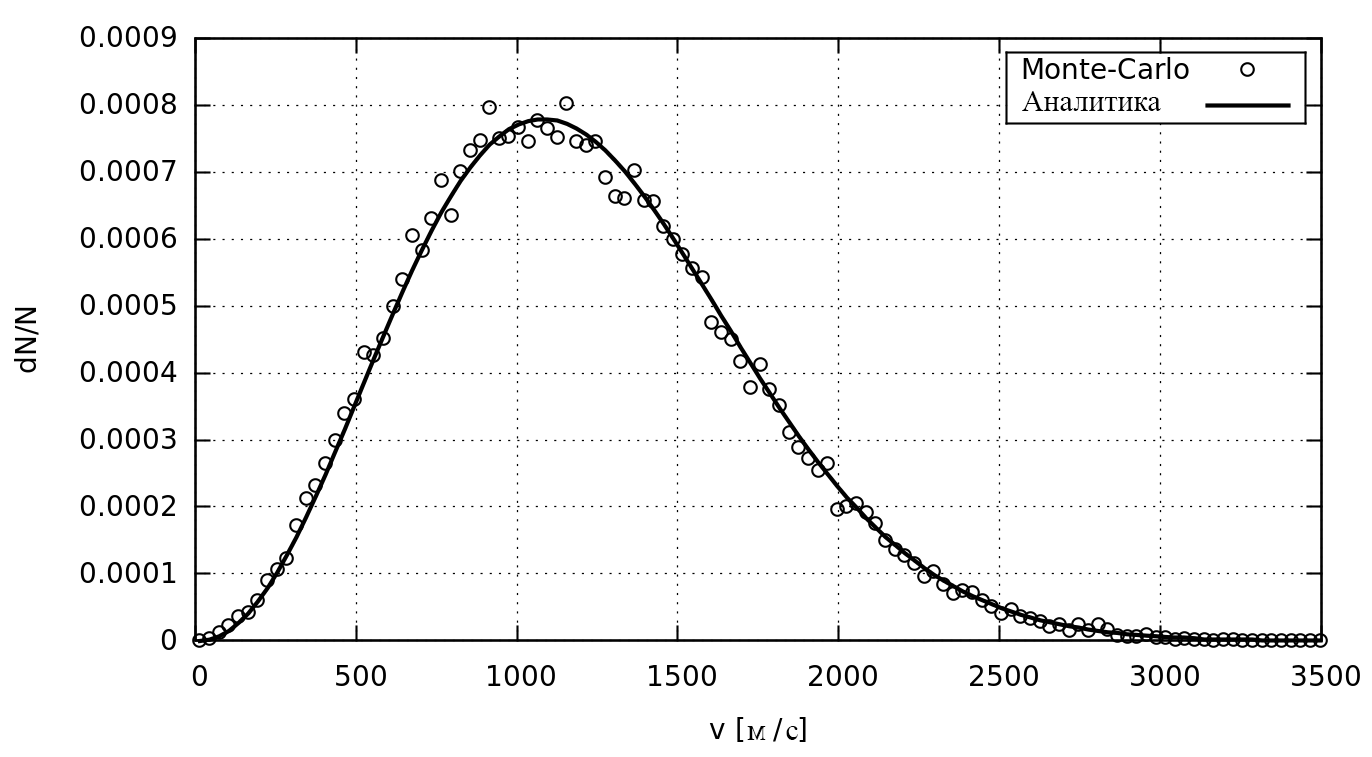
\includegraphics[width=0.85\linewidth]{./fig/ch4/He(T=273)}
\caption{Проверка процедуры задания случайной величины по распределению Максвелла для гелия при $T = 273 \text{ К}$}
\label{fig:He(T=273)}
\end{figure}


\section{Интегрирование уравнения движения для одной частицы}

Для решения \eqref{eq:style1} и \eqref{eq:style2} с помощью метода Рунге-Кутты используется код написанный на языке \texttt{c++}.
Перед моделированием достаточно сложных процессов необходимо выяснить насколько точно и правильно считает программа.
Для этого следует численно решить те задачи, которые имеют аналитическое решение.

\subsection{Движение в постоянном однородном электрическом поле.}

Рассмотрим электрон
\begin{equation*}
m = m_e = 9.10938291 \cdot 10^{-31} \text{ кг}, \qquad q = -e = - 1.60217657 \cdot 10^{-19} \text{ Кл}
\end{equation*}
 в поле
$
\vec{E} = E \vec{e}_x
,\ 
E = 10\ \dfrac{\text{кВ}}{\text{м}}$. Пусть в момент времени $t=0$
\begin{equation*}
\vec{r}(0) = 0, \qquad \vec{v}(0) = v_0 \vec{e}_y, \qquad v_0 = 0,8c.
\end{equation*}
Время моделирования --- $T = 1 \text{ мс}$. Данная задача решается аналитически для релятивистского случая. Явная зависимость координат частиц от времени тогда задаётся выражениями
\begin{equation}
	\begin{cases}
		x(t) = \dfrac{1}{qE} \left(\sqrt{\mathscr{E}_0^2 + (cqEt)^2 } - \mathscr{E}_0 \right),  \\ \\
		y(t) = \dfrac{p_0c}{qE} \Arsh \dfrac{cqEt}{\mathscr{E}_0},
	\end{cases}
	\label{eq:analytical1}
\end{equation}
где $\mathscr{E}_0  = \sqrt{m^2c^4 + c^2 p_0^2}$ имеет смысл энергии частицы при $t = 0$; а $p_0 = m_e v_0 / \sqrt{1 - v^2_0/c^2}$.
Траектория частицы будет представлять собой цепную линию.


Сравнение аналитического решения \eqref{eq:analytical1} с результатом численного эксперимента представлено на рис. \ref{fig:Eonly}.

\begin{figure}[h]
\centering
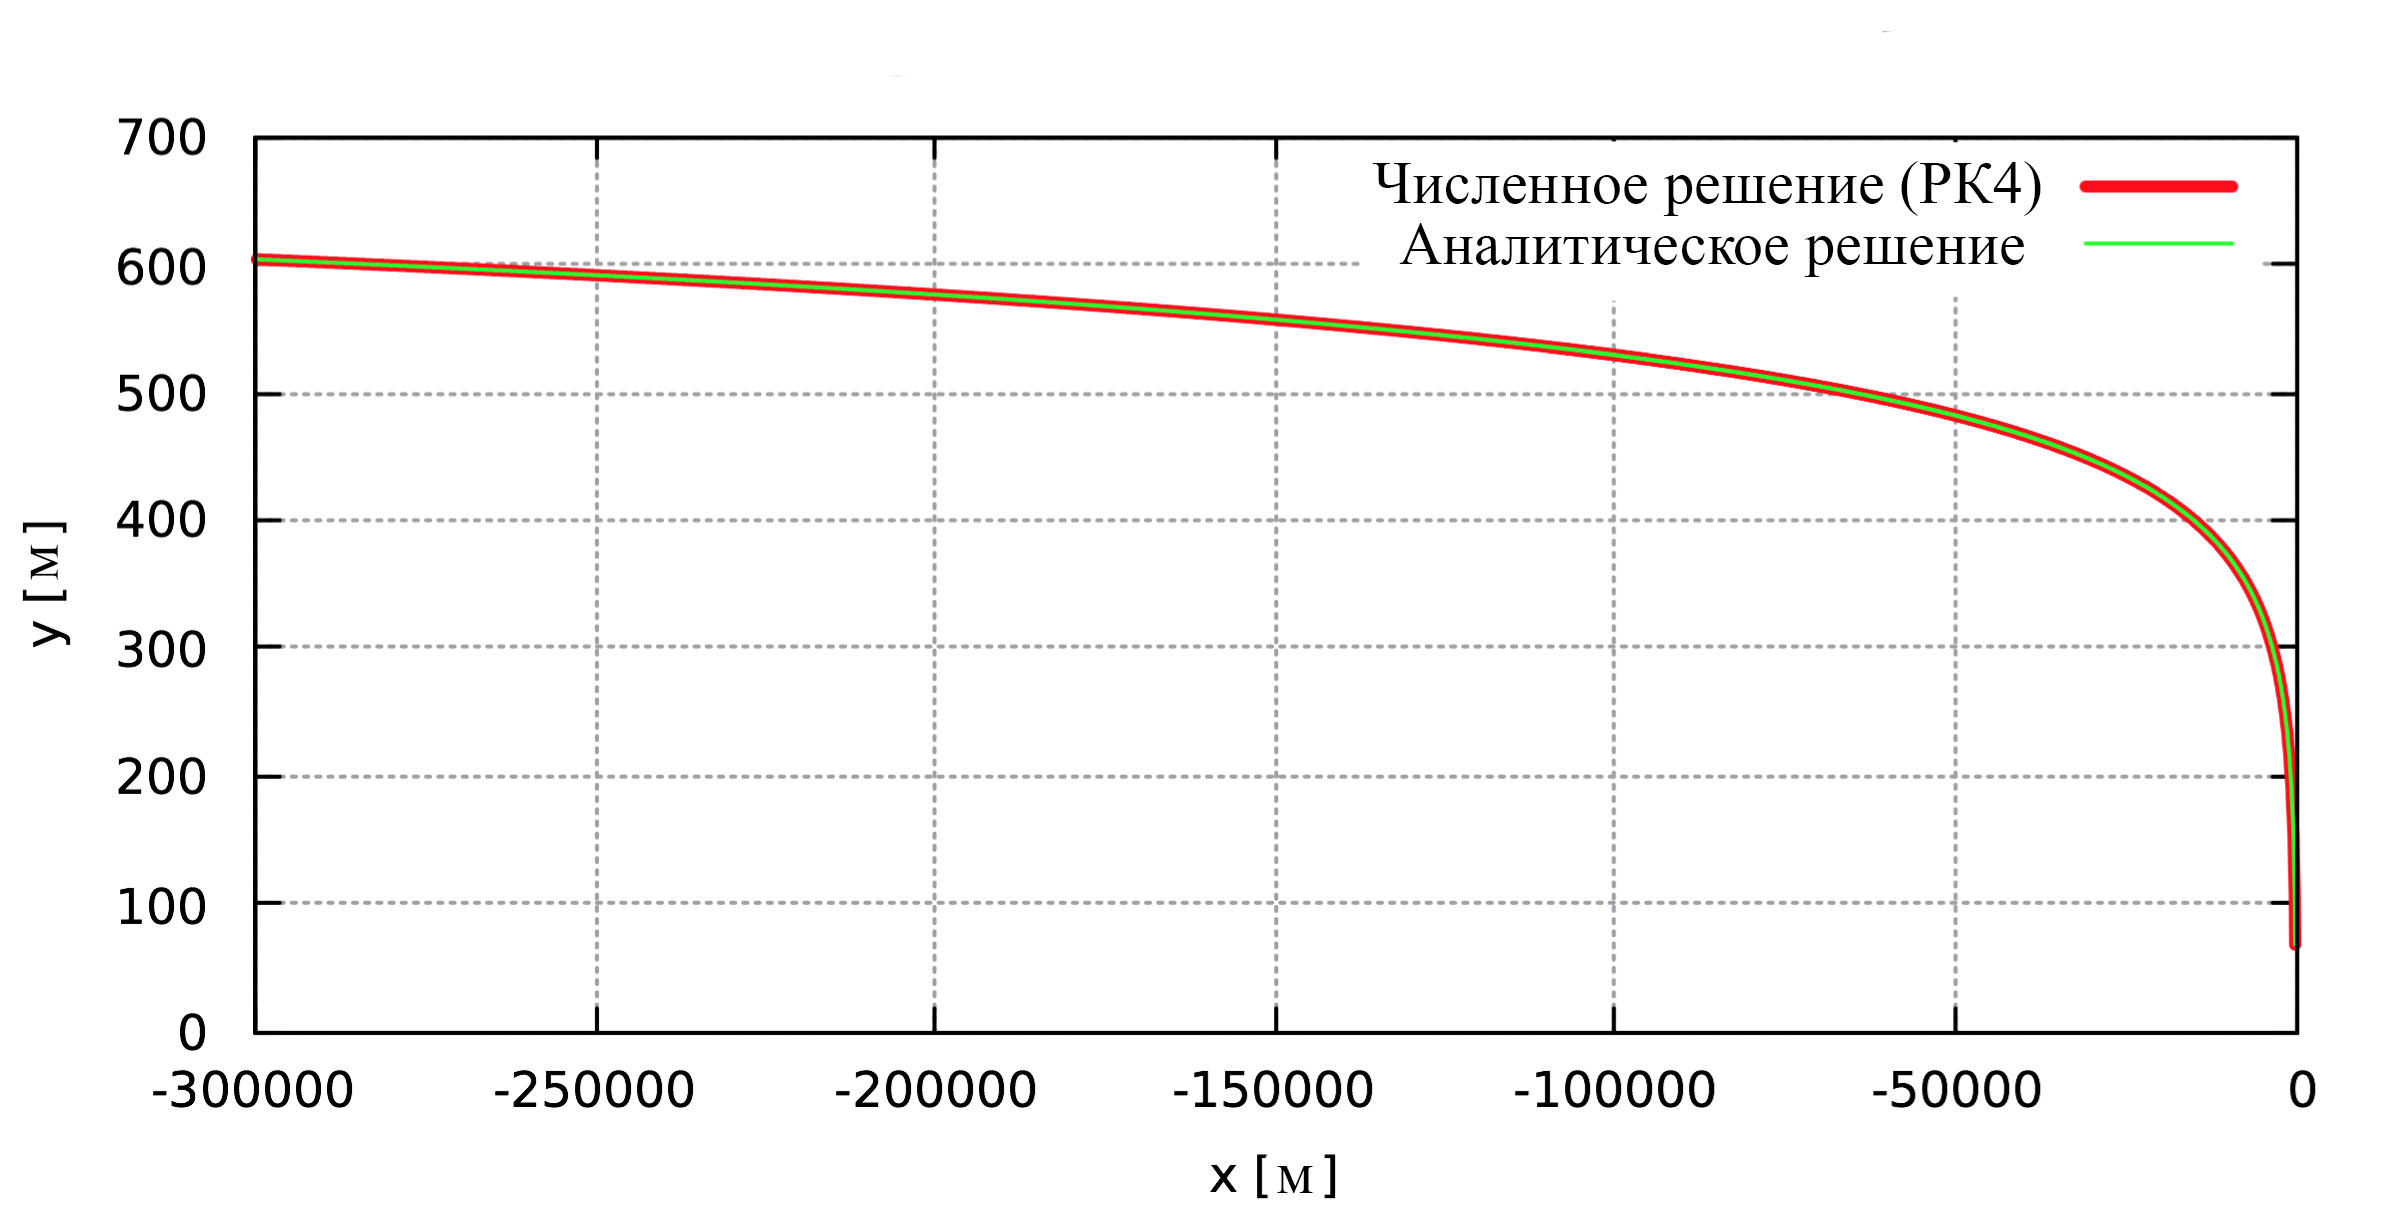
\includegraphics[width=.9\textwidth]{ch4/Eonly.png}
\caption{Моделирование движения электрона в однородном электрическом поле}
\label{fig:Eonly}
\end{figure}

В зависимости от различных значений $dt$, метод Рунге-Кутты сходится по разному. Из-за машинной ошибки ЭВМ принцип чем меньше $dt$, тем точнее результат оказывается неверен. Это явно видно на рис. \ref{fig:errors}, где представленная зависимость вида 
\begin{equation*}
err(t) = \sqrt{ [x^{\text{an}}(t) - x^{\text{num}}(t) ]^2  + [y^{\text{an}}(t) - y^{\text{num}}(t)]^2 }.
\end{equation*}


\begin{figure}[h]
	\begin{minipage}[h]{.33\linewidth}
	\center{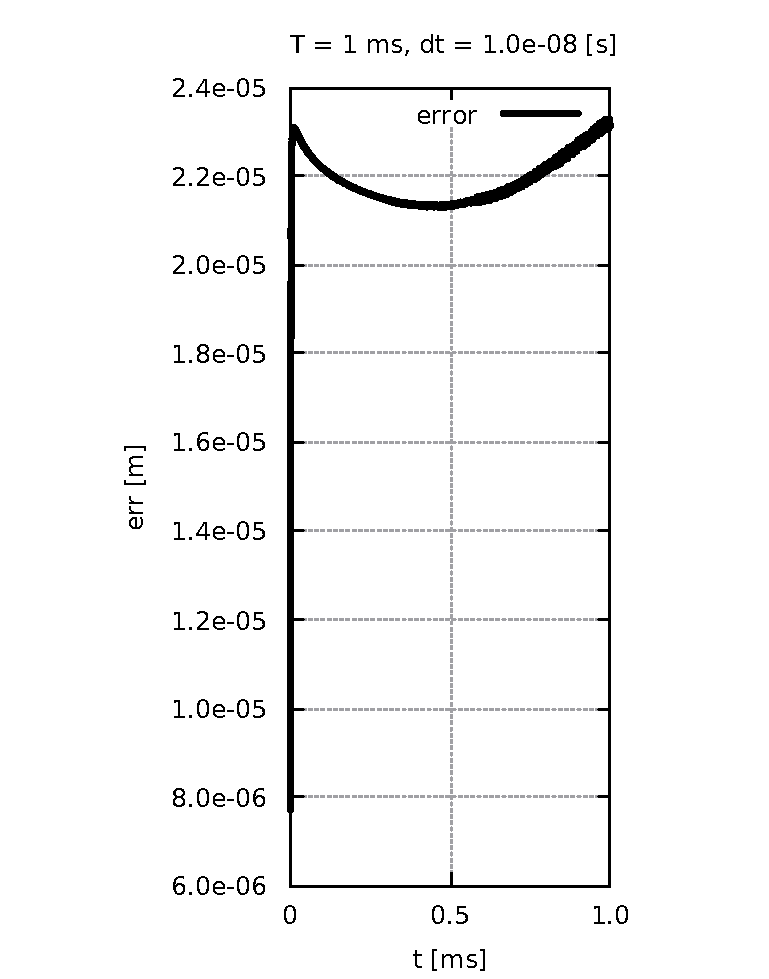
\includegraphics[width=1.14\linewidth]{ch4/err-dt-8} }
	\end{minipage}
	\hfill
	\begin{minipage}[h]{.33\linewidth}
	\center{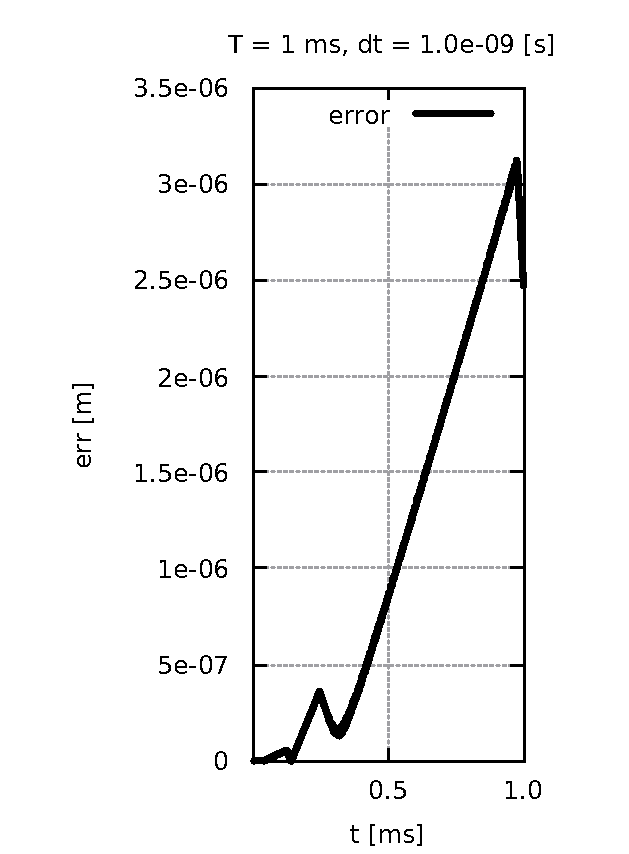
\includegraphics[width=1.1\linewidth]{ch4/err-dt-9} }
	\end{minipage}
	\hfill
	\begin{minipage}[h]{.32\linewidth}
	\center{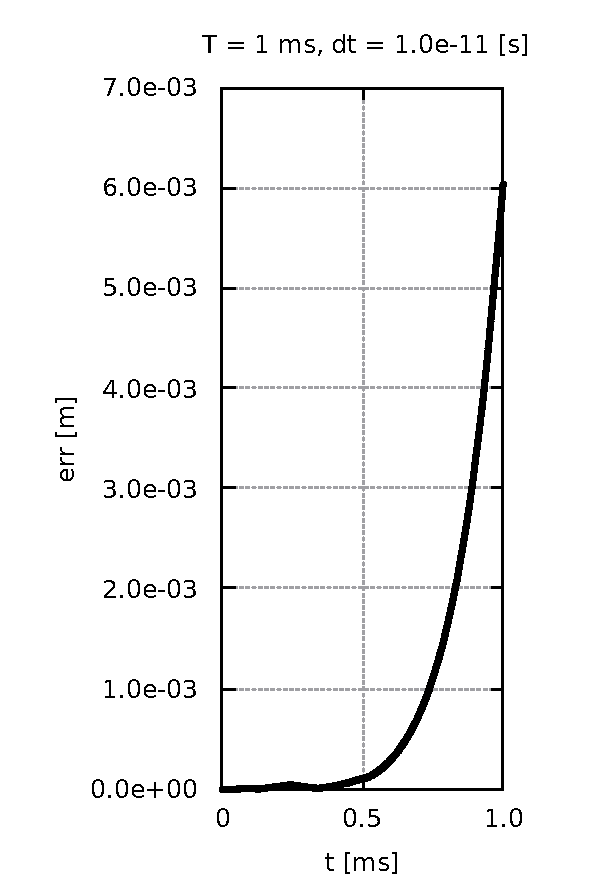
\includegraphics[width=1.02\linewidth]{ch4/err-dt-11} }
	\end{minipage}
	\caption{Расходимость решения при различных $dt$ при моделировании движения электрона в однородном электрическом поле методом Рунге-Кутты}
	\label{fig:errors}
\end{figure}

Оценим точность выбранного метода. За время $T = 1 \text{ мс}$ (достаточно большее временной промежуток для электронных приборов) электрон пролетел путь примерно в $300 \text{ км}$, что, разумеется много больше, чем любое электронное устройство, созданное человеком. Отклонение от траектории по сравнению с пройденным расстоянием составляет всего $$\dfrac{10^{-6} \text{ м}}{3\cdot10^5 \text{ м}} \approx 10^{-11} = 10^{-9} \%.$$

\subsection{Движение во взаимно перпендикулярных постоянных однородных электрическом и магнитном полях.}

Рассмотрим движение позитрона 
\begin{equation*}
m = m_e = 9.10938291 \cdot 10^{-31} \text{ кг}, \qquad q = +e = 1.60217657 \cdot 10^{-19} \text{ Кл}
\end{equation*}
в поле 
\begin{eqnarray*}
\vec{E} = E  \vec{e}_y, &\qquad& \vec{B} = B  \vec{e}_z, \\ \\
E = 10\ \frac{\text{кВ}}{\text{м}}, &\qquad& B = \frac{E}{c} \approx 33,4\ \text{мкТл}.
\end{eqnarray*}
В момент времени $t = 0$
\begin{eqnarray*}
\vec{r}(0) = 0, \qquad v_0 = 0,8c, \\ \\
 \vec{v}(o) = v_0 \cos \left( \frac{\pi}{4}\right) \vec{e}_x + v_0 \sin \left( \frac{\pi}{4}\right) \vec{e}_z.
\end{eqnarray*}
Тогда импульс частицы можно найти как
\begin{eqnarray*}
p_{0x} = \frac{m_e (\vec{v} \cdot \vec{e}_x) }{\sqrt{1 - v_0^2/c^2}}, &\qquad& p_{z} = \frac{m_e (\vec{v} \cdot \vec{e}_z) }{\sqrt{1 - v_0^2/c^2}}, \\ \\
p_{0x} \approx 2.57\cdot 10^{-22}\ \frac{\text{кг} \cdot \text{м}}{\text{с}}, &\qquad& p_{z} \approx 2.57\cdot 10^{-22}\ \frac{\text{кг} \cdot \text{м}}{\text{с}}.
\end{eqnarray*}

Аналитическое решение данной задачи сложно, но выполнимо \cite{Landau2}. В общем виде решение записывается следующим образом:
\begin{eqnarray}
2qEt &=& \frac{c^2}{3 \alpha^2} p_y^3  + \left(  1 + \frac{\xi^2}{\alpha^2}  \right) p_y, \label{eq:ans00} \\
x &=& \frac{c}{2qE} \left( \frac{\xi^2}{\alpha^2}  - 1  \right) p_y + \frac{c^3}{6qE \alpha^2} p_y^3, \label{eq:ans01} \\
y &=& \frac{c^2}{2 \alpha q E} p_y^2, \label{eq:ans02} \\
z &=& \frac{p_z c^2}{qE \alpha} p_y, \label{eq:ans03}
\end{eqnarray}
где $\xi^2 = m^2 c^4 + c^2 p_z^2 = \const$; $\alpha = \varepsilon - cp_x$; а $\varepsilon = mc^2/ \sqrt{1 - v^2/c^2}$.
Рассмотрим выражение \eqref{eq:ans00} в рамках данной задачи. Перепишем его в виде:
\begin{equation}
t(p_y) =  \frac{c^2}{6eE\alpha^2} p_y^3 + \frac{(1 + \xi^2/\alpha^2)}{2 e E} p_y.
\label{eq:t_py}
\end{equation}

\begin{figure}[h]
	\centering
	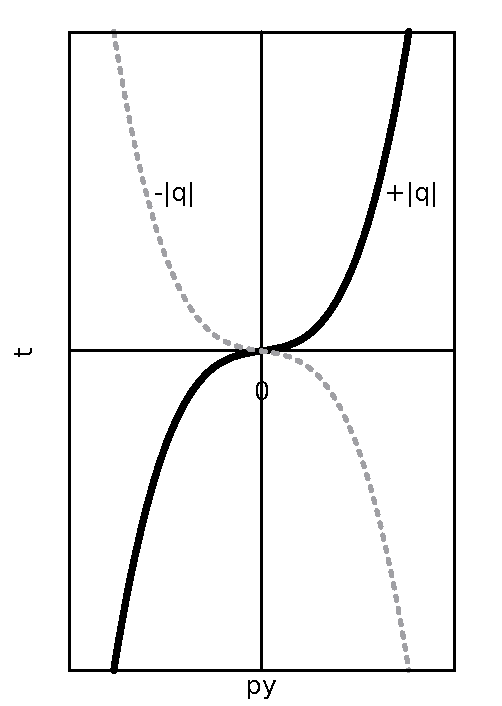
\includegraphics[width=.3\textwidth]{ch4/t_py}
	\caption{Зависимость $t(p_y)$ для положительного и отрицательного заряда}
	\label{fig:t_py}
\end{figure}

Видно, что коэффициент при $p_y$ в любом случае одного знака, в данном случаи оба положительны. Тогда у кривой $t = t(p_y)$ будет только один вещественный корень (рис. \ref{fig:t_py}). Кроме того, с увеличением $t$ импульс $p_y$ будет увеличиваться. Таким образом, можно заключить, что в интересующей нас области возможно однозначно выразить $p_y = p_y(t)$. Перепишем уравнение \eqref{eq:t_py} в следующем виде:
\begin{equation*}
p_y^3 + A p_y - B t = 0,
\end{equation*}
где
\begin{equation*}
A =  \frac{3 \alpha^2 (1 + \xi^2/\alpha^2)}{c^2}, \qquad B = \frac{6\alpha^2eE}{c^2}.
\end{equation*}
Выполним подстановку\cite{bronshtein-math} вида
\begin{equation*}
p_y = w - \frac{A}{3 w},
\end{equation*}
получим
\begin{equation*}
w^6 - Bt w^3 - \frac{A^3}{27} = 0.
\end{equation*}
Его решение:
\begin{equation}
w^3_{1,2} = \frac{ Bt \pm \sqrt{B^2 t^2 + \frac{4}{27}A^3}}{2}.
\label{eq:solve_go_tusk}
\end{equation}
Как уже говорилось выше, должна выполняться асимптотика вида 
$$\lim\limits_{t \to + \infty} p_y(t) =  +\infty, $$ 
тогда, очевидно, следует выбрать знак <<$+$>> в решении \eqref{eq:solve_go_tusk}. Запишем 
\begin{equation*}
p_y(t) = \sqrt[3]{\frac{Bt}{2} + \sqrt{\frac{B^2 t^2}{4} + \frac{A^3}{27}}} - \frac{A}{3 \sqrt[3]{\frac{Bt}{2} + \sqrt{\frac{B^2 t^2}{4} + \frac{A^3}{27}}}}
\end{equation*}
или подставив значения констант $A$ и $B$, получим:
%\begin{equation}
%w^3 = \frac{3 \alpha^2 eE}{c^2}t + \frac{\alpha^2}{c^3} \sqrt{9 e^2 E^2c^2t^2 + \alpha^2  \left( 1 + \xi^2/\alpha^2  \right)^3  }
%\end{equation}
%\begin{multline}
%p_y(t) = \sqrt[3]{\frac{3 \alpha^2 eE}{c^2}t + \frac{\alpha^2}{c^3} \sqrt{9 e^2 E^2c^2t^2 + \alpha^2  \left( 1 + \xi^2/\alpha^2  \right)^3  }} -\\-
%\frac{ \left( \alpha^2 + \xi^2  \right)  }{c^2\sqrt[3]{\frac{3 \alpha^2 eE}{c^2}t + \frac{\alpha^2}{c^3} \sqrt{9 e^2 E^2c^2t^2 + \alpha^2  \left( 1 + \xi^2/\alpha^2  \right)^3  }}}
%\end{multline}

\begin{multline}
p_y(t) = \sqrt[3]{\frac{3 \alpha^2 eE}{c^2}t + \frac{\alpha^2}{c^3} \sqrt{9 e^2 E^2c^2t^2 + \alpha^2  \left( 1 + \xi^2/\alpha^2  \right)^3  }} -\\-
\frac{ \left( \alpha^2 + \xi^2  \right)  }{\sqrt[3]{3 \alpha^2c^4 eEt + \alpha^2c^3 \sqrt{9 e^2 E^2c^2t^2 + \alpha^2   \left( 1 + \xi^2/\alpha^2  \right)^3  }}}
\label{eq:phyco}
\end{multline}
Подставляя \eqref{eq:phyco} в \eqref{eq:ans01}, \eqref{eq:ans02}и \eqref{eq:ans03} получим аналитическое решение вида $\vec{r} = \vec{r}(t)$.

Промоделируем движение позитрона в течении $T = 1 \text{ мс}$ и сравним результат с аналитическим выражением (рис. \ref{fig:xyz_EB}).


\begin{figure}[h]
	\begin{minipage}[h]{.70\linewidth}
	\center{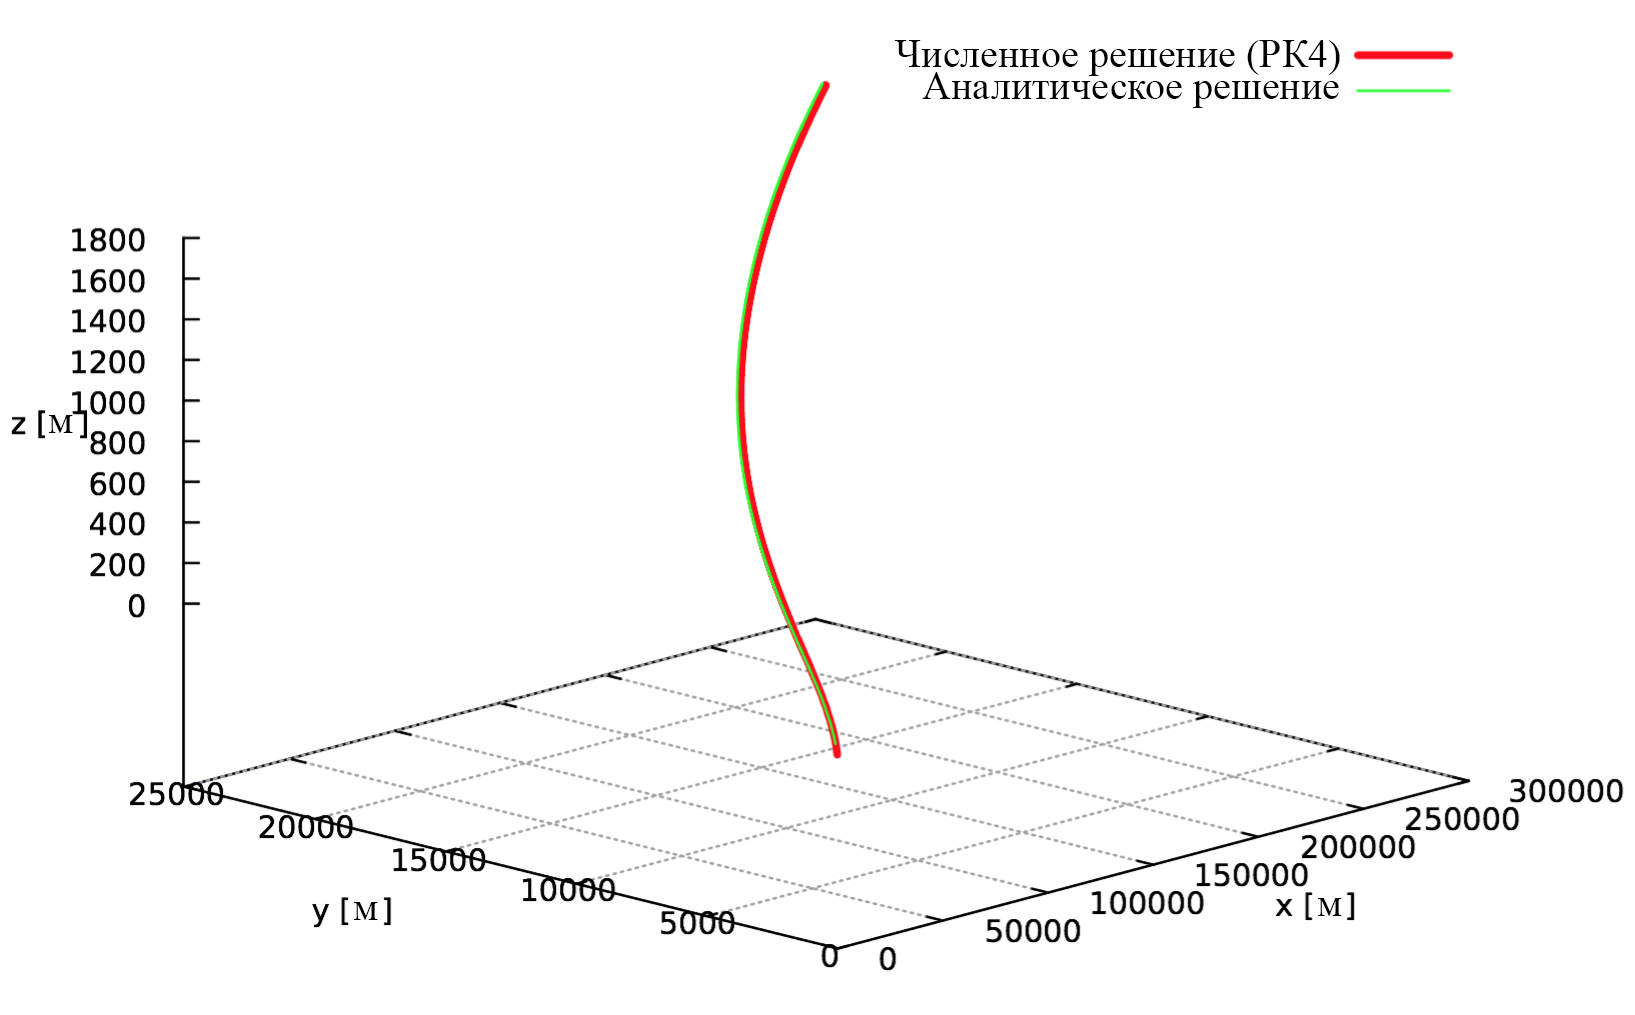
\includegraphics[width=1.\linewidth]{ch4/xyz_EB.png} }{ а) \\}
	\end{minipage}
	\hfill
	\begin{minipage}[h]{.29\linewidth}
	\center{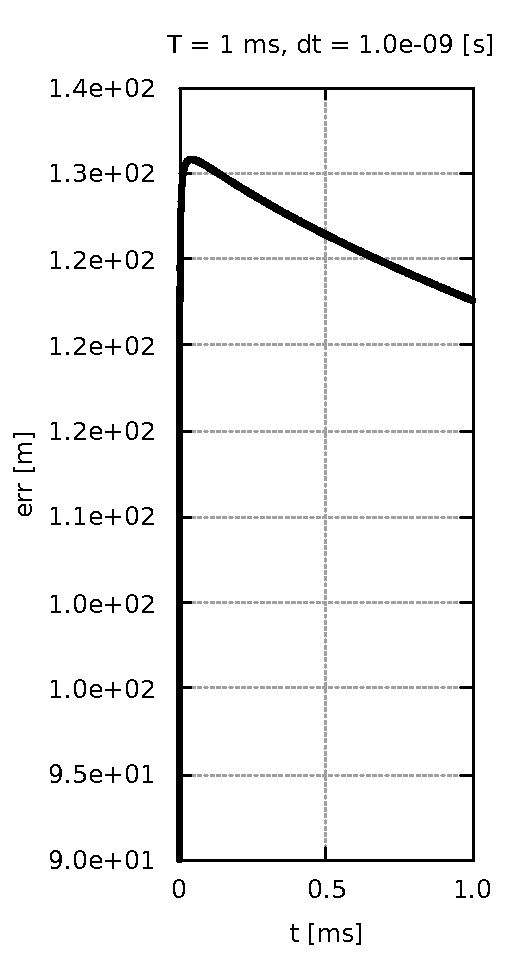
\includegraphics[width=1.\linewidth]{ch4/err-xyz} }{ б) \\} 
	\end{minipage}
	\caption{Аналитическое и численное решения уравнения движения позитрона: a) траектория позитрона; б) ошибка решения}
	\label{fig:xyz_EB}
\end{figure}


\subsection{Определения приемлемых параметров вычисления}


Поставим задачу определить временную дискретизацию  численного решения, которая обеспечит необходимую точность расчёта. 

В качестве характерных заряженных частиц в плазме выбраны:
\begin{enumerate}
\item Электрон:
\begin{equation*}
m_e = 9,109 \cdot 10^{-31} \text{ кг}, \qquad q_e = - |e| = - 1,602 \cdot 10^{-19} \text{ Кл}.
\end{equation*}

\item Тритон:
\begin{equation*}
m_T = 5,007 \cdot 10^{-27} \text{ кг}, \qquad q_T = + |e| = + 1,602 \cdot 10^{-19} \text{ Кл}.
\end{equation*}

\end{enumerate}

Характерные размеры магнитных ловушек лежат в диапазоне \cite{dimov2005}

\begin{equation}
L = 0,5 \div 6 \text{ м.}
\end{equation}
Это значит, что заряженная частица, пролетев данное характерное расстояние $L$ не должна значительно отклониться от истинной траектории.


Положим в пространстве однородное скрещенное электромагнитное поле:
\begin{equation}
\vec{E} = E  \vec{e}_y, \qquad \vec{B} = B  \vec{e}_z.
\end{equation}
Типовые значения магнитной индукции в различных ловушках, как было выяснено в главе \ref{ch1}, следующие
\begin{equation}
B \sim 0,1 \div 3 \text{ Тл}.
\end{equation}

\subsubsection{Движение электрона}

Рассмотрим движение электрона. Переносную скорость выберем релятивистской (частицы в <<хвосте>> распределения Максвелла)
\begin{equation}
v_{tr} = \frac{E}{B} = 0,8c.
\end{equation}
При данных параметрах была проведена серия численных экспериментов для электрона (рисунок \ref{fig:dt_11}, \ref{fig:dt_12}). Таким образом, можно сделать первую оценку для шага по времени:
\begin{equation}
dt \leqslant 10^{-12} \text{ с}.
\end{equation}


\begin{figure}[h!]
\centering
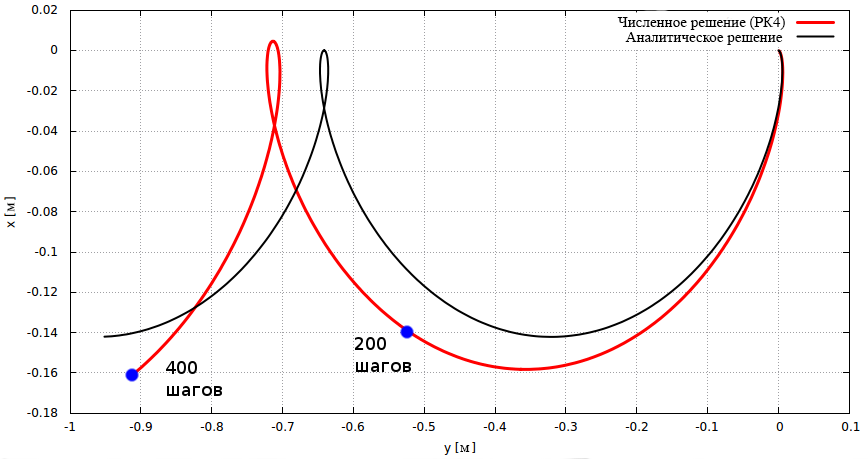
\includegraphics[width=0.8\linewidth]{./fig/ch4/dt_11}
\caption{Движение электрона в скрещенных полях при $B = 0,1$ Тл, $v_{tr} = 0,8 c$ и $dt = 10^{-11}$ с}
\label{fig:dt_11}
\end{figure}
\begin{figure}[h!]
\centering
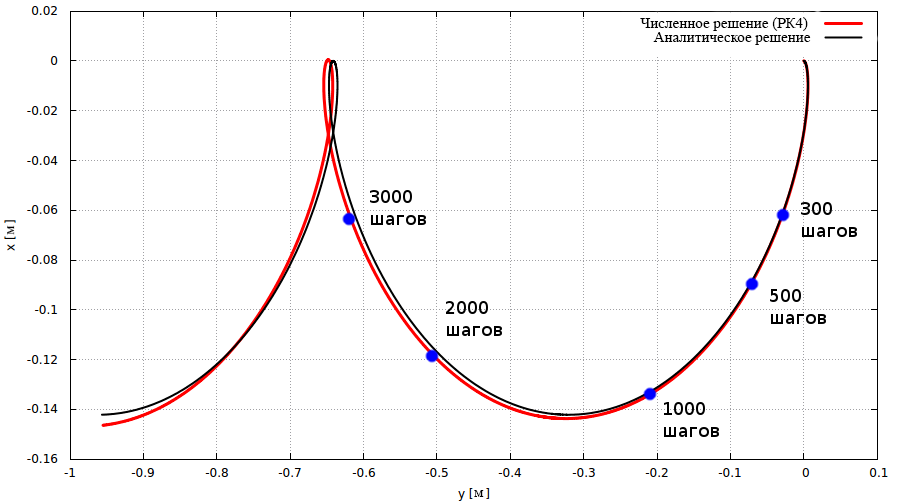
\includegraphics[width=0.8\linewidth]{./fig/ch4/dt_12}
\caption{Движение электрона в скрещенных полях при $B = 0,1$ Тл, $v_{tr} = 0,8 c$ и $dt = 10^{-12}$ с}
\label{fig:dt_12}
\end{figure}

Релятивизм у электрона проявляется достаточно сильно в силу его малой массы, а значит и малого ларморовского радиуса. На заданных масштабах могут происходить сильные отклонения от истинной траектории. Численные эксперименты показывают, что необходимо уже учитывать эффекты релятивизма уже  при $v \gtrsim 0,01 c$. При более высоких скоростях расхождение между нерелятивистским и релятивистским решениями уже очень велико (рисунок \ref{fig:electron_very_fast}).

\begin{figure}[h!]
\centering
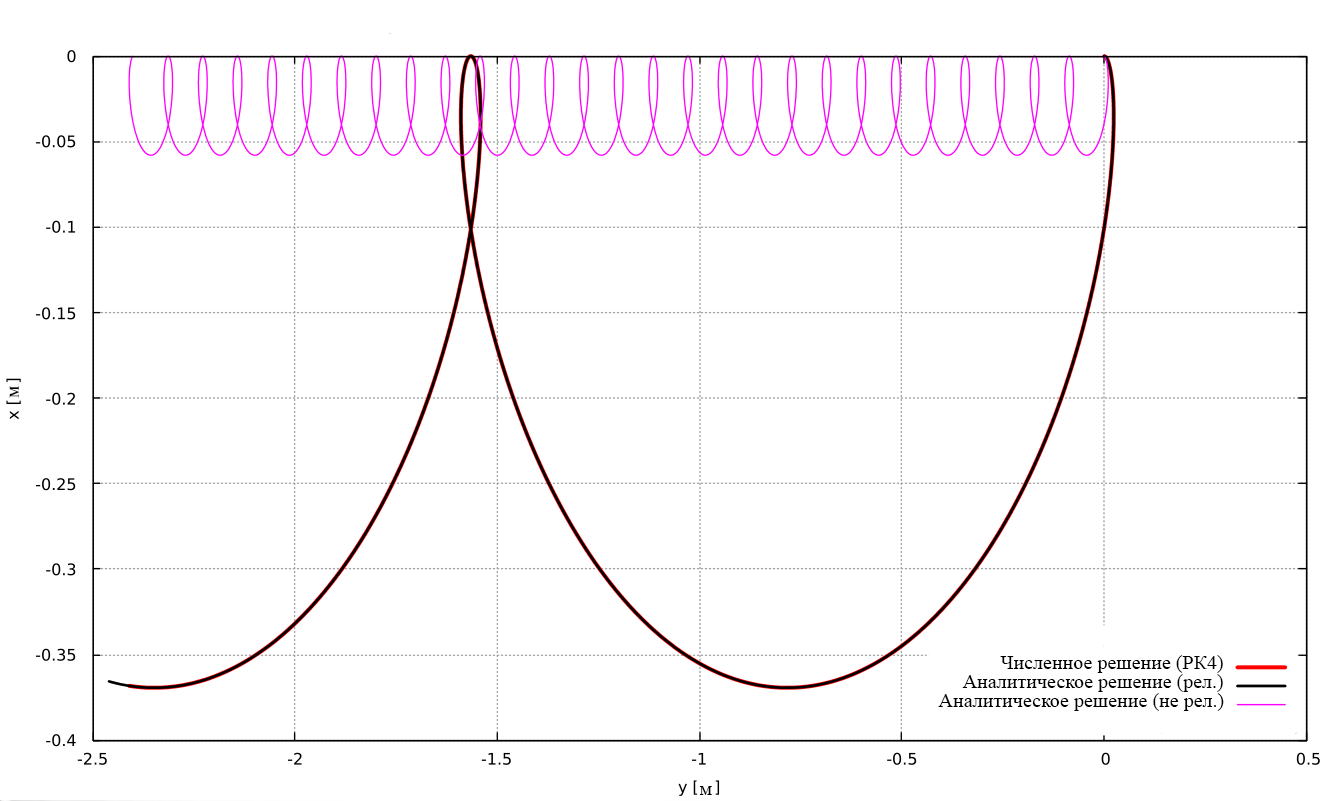
\includegraphics[width=0.9\linewidth]{./fig/ch4/electron_very_fast.png}
\caption{Движение электрона в скрещенных полях. $B = 0,1 \text{ Тл}$, $v_{tr} = 0,8 c$, $v_0 = 0,9 c$. На графике представлены три решения: одно численное и два аналитических (релятивистское и нерелятивистское). Шаг по времени --- $dt = 10^{-15}$}
\label{fig:electron_very_fast}
\end{figure}





\subsubsection{Движение иона}

В случае движения иона, а конкретно тритона, ситуация иная. На заданных масштабах ощутимый вклад в отклонения вносит именно начальная скорость частицы. В пределах $10\div50 \text{ м}$ можно получить нерелятивистскую траекторию, которая будет достаточно точна (рис. \ref{fig:triton}).

\begin{figure}
\centering
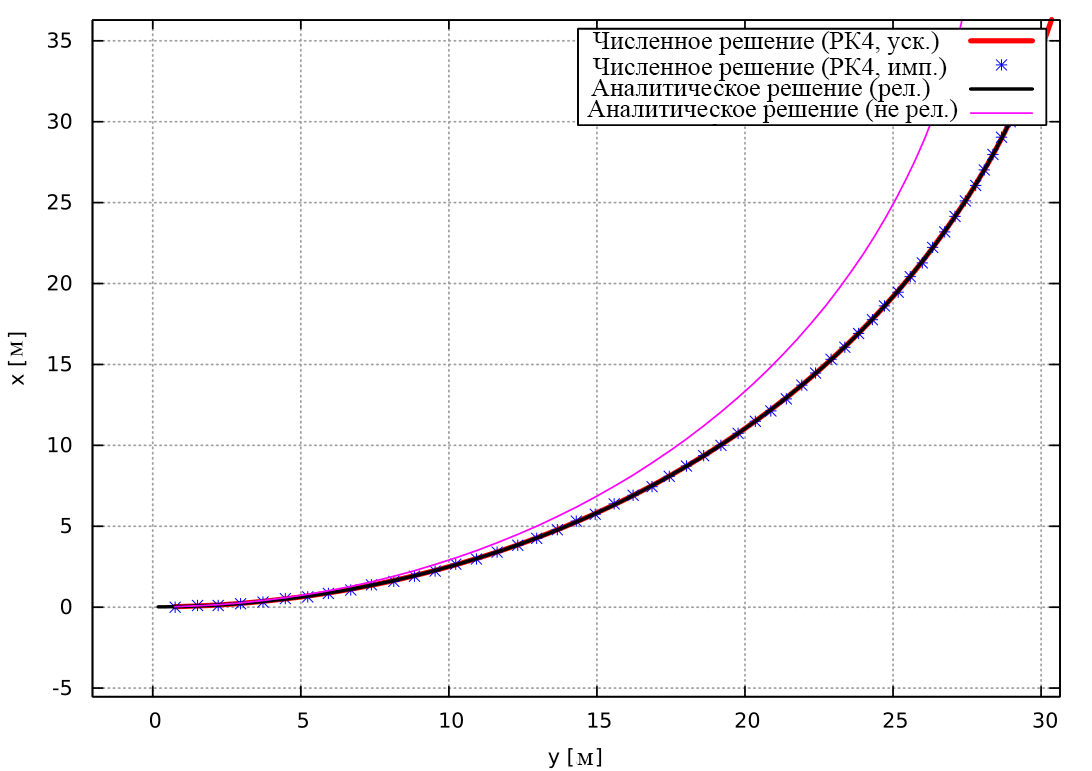
\includegraphics[width=.8\linewidth]{./fig/ch4/triton}
\caption{Движение тритона в скрещенных полях. $B = 0,1 \text{ Тл}$, $v_{tr} = 0,8 c$, $v_0 = 0,5 c$. На графике представлены 4 решения: два численных и два аналитических (релятивистское и нерелятивистское). Шаг по времени --- $dt = 10^{-13}$}
\label{fig:triton}
\end{figure}



\section{Проверка достоверности вычислительной программы для моделирования большого числа частиц}

Точное описание группы (ансамбля) релятивистских заряженных частиц является гораздо более сложной вычислительной задачей. Это обусловлено конечной скоростью передачи взаимодействия. Для того, чтобы это учесть вводятся запаздывающие потенциалы Лиенара-Вихерта, из которых получаются выражения для полей \eqref{eq:opt_LV_B_early} и \eqref{eq:opt_LV_E_early}, которые учитывают <<прошлое>> системы. 
С точки зрения ЭВМ это обозначает, что необходимо держать в памяти программы \textit{всю предысторию} вычисляемой задачи.
Аналитически же задачу решить не возможно, т.~к. задача о трёх телах уже не решаема. 

Проверка адекватности полученных результатов проводилась путём сравнения с независимыми численными экспериментами других исследователей, результаты которых освещены в печати \cite{kd2004,Kovtun2005,Kovtun2010,Kravchenya2010}.

Результаты сравнения представлены на рисунке \ref{fig:check1}. Кроме того, был выяснен порог количества крупных частиц, при котором качественный вид картины искажается (рисунок \ref{fig:check2}).


\begin{figure}[h!]
\begin{minipage}[h]{0.9\linewidth}
\center{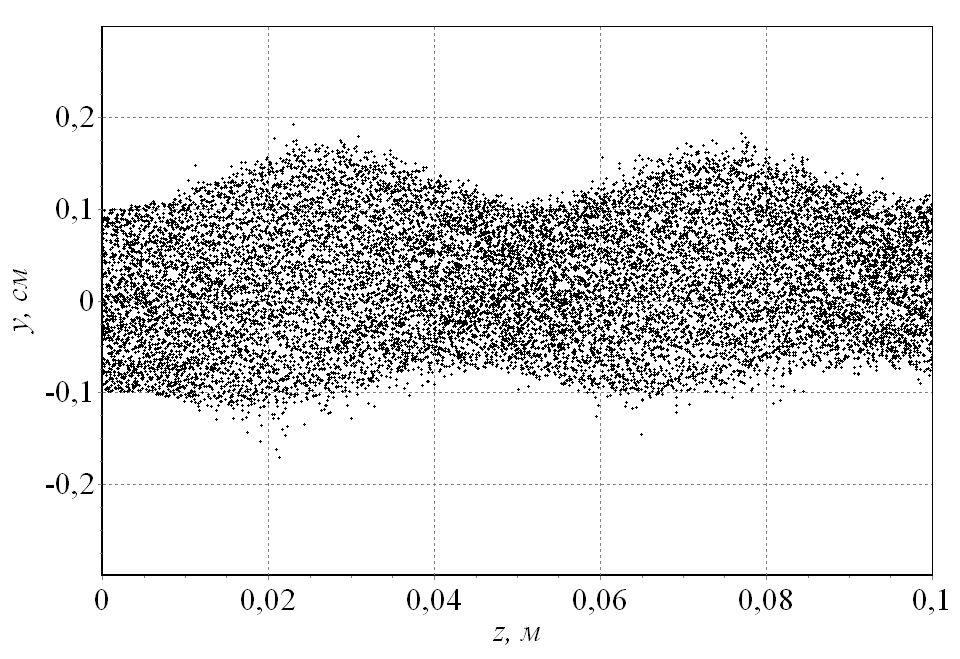
\includegraphics[width=1\linewidth]{ch4/Hegai-ZOY-b}} а) Из работы \cite{kd2004} \\
\end{minipage}
\vfill
\begin{minipage}[h]{0.9\linewidth}
\center{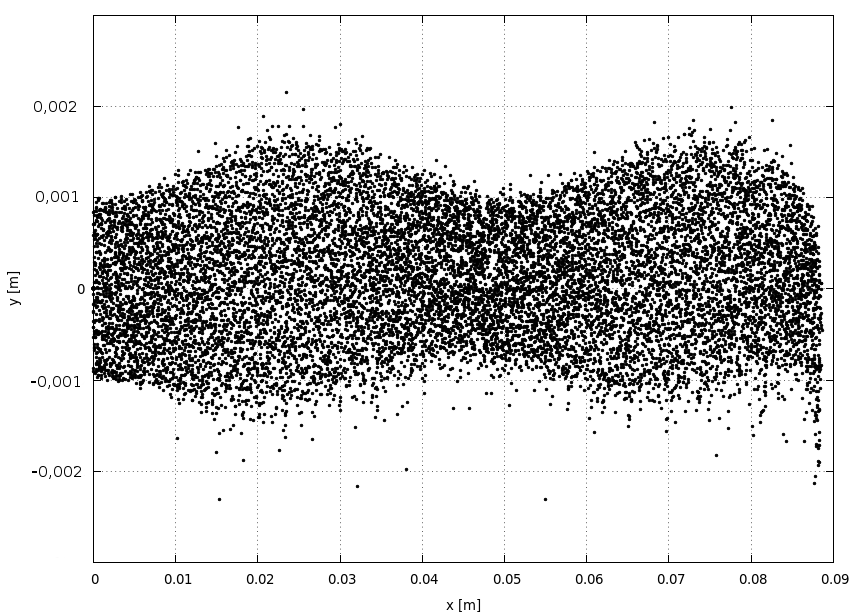
\includegraphics[width=1\linewidth]{ch4/YoZ}} б) Из составленной модели  \\
\end{minipage}
\caption{Проверка полученной модели на адекватность результатов. Параметры потока: $dt = 10^{-12}$ с, $v_0 = v_{tr} = 0,8 c$, плотность зарядов на влёте $\rho = 0,1 \ \frac{\text{Кл}}{\text{м}^3}$, $B = 0,5$ Тл, общее количество частиц $N \approx 20000$}
\label{fig:check1}
\end{figure}

\begin{figure}[h!]
\begin{minipage}[h]{0.45\linewidth}
\center{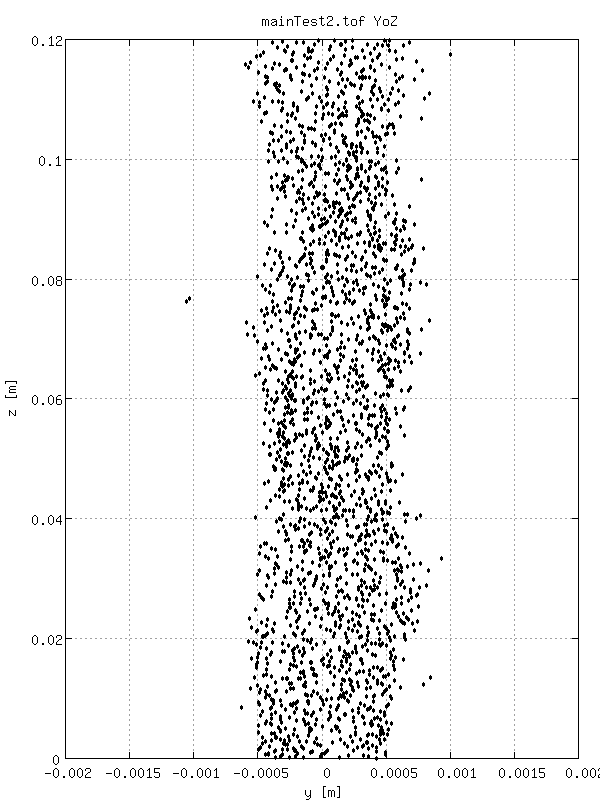
\includegraphics[width=1\linewidth]{ch4/mainTest2-tof_YoZ.png}} а) $N = 3000$ \\
\end{minipage}
\hfill
\begin{minipage}[h]{0.45\linewidth}
\center{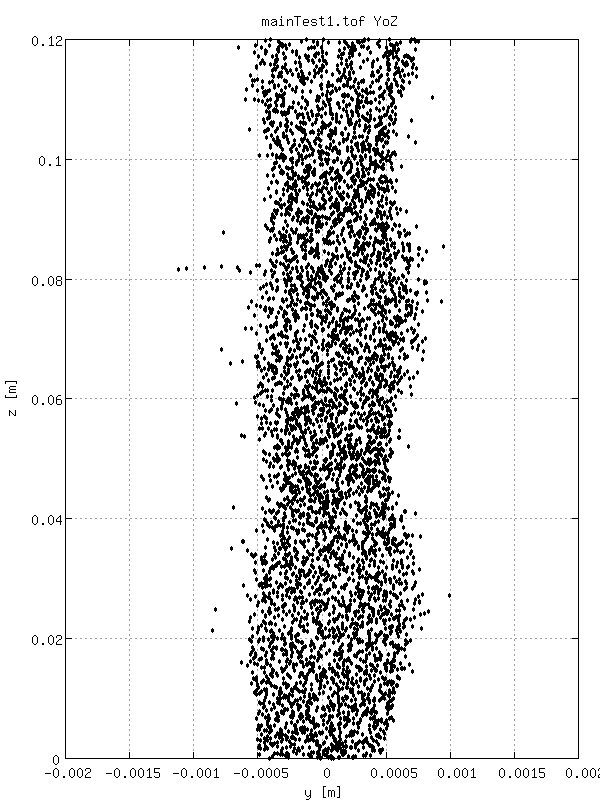
\includegraphics[width=1\linewidth]{ch4/mainTest1-tof_YoZ.png}} б) $N = 9000$ \\
\end{minipage}
\caption{Изменение количества моделируемых частиц $N$ в релятивистском потоке. Параметры потока: $dt = 10^{-12}$ с, $v_0 = v_{tr} = 0,8 c$, плотность зарядов на влёте $\rho = 0,05 \ \frac{\text{Кл}}{\text{м}^3}$, $B = 0,5$ Тл}
\label{fig:check2}
\end{figure}


